\documentclass[]{article}
\usepackage{blindtext, graphicx}
\usepackage{float}

%opening
\title{Lab 2: Autonomous Vehicles}
\author{Ethan Puerto}

\begin{document}
\maketitle
\newpage
\tableofcontents


\newpage
\section{Block Diagram}
\begin{figure}[h]
	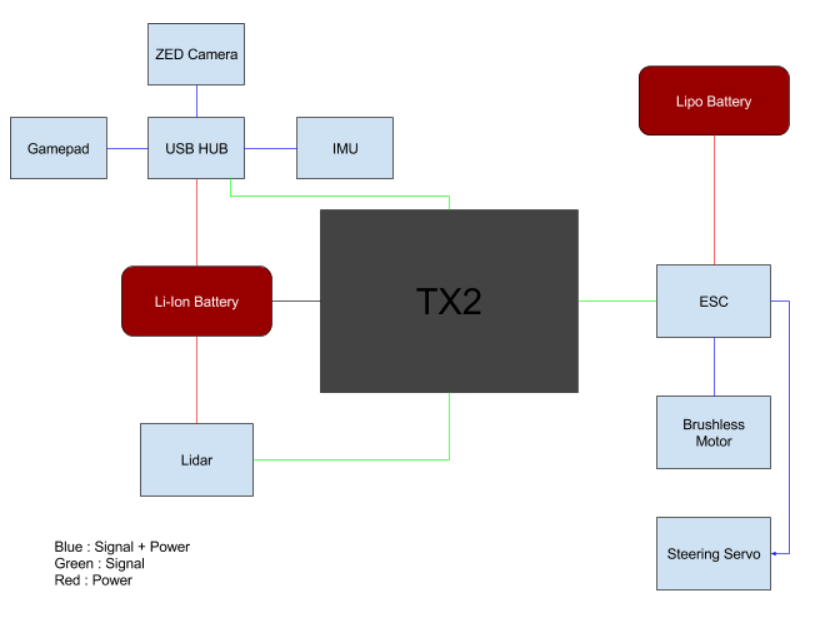
\includegraphics[width=12cm]{blockdiagram}
	\centering
\end{figure}

\newpage
\section{Car Specifications}

\begin{table}[H]
	\centering
	\begin{tabular}{lll}
		\textit{\textbf{TX2}}             &                                                                  &  \\
		\textit{GPU}                      & NVIDIA Pascal™, 256 CUDA cores                                   &  \\
		\textit{CPU}                      & HMP Dual Denver 2/2 MB L2 +Quad ARM® A57/2 MB L2                 &  \\
		\textit{Video}                    & 4K x 2K 60 Hz Encode (HEVC)4K x 2K 60 Hz Decode (12-Bit Support) &  \\
		\textit{Memory}                   & 8 GB 128 bit LPDDR459.7 GB/s                                     &  \\
		\textit{Display}                  & 2x DSI, 2x DP 1.2 / HDMI 2.0 / eDP 1.4                           &  \\
		\textit{CSI}                      & Up to 6 Cameras (2 Lane)CSI2 D-PHY 1.2 (2.5 Gbps/Lane)           &  \\
		\textit{PCIE}                     & Gen 2 | 1x4 + 1x1 OR 2x1 + 1x2                                   &  \\
		\textit{Data Storage}             & 32 GB eMMC, SDIO, SATA                                           &  \\
		\textit{Other}                    & CAN, UART, SPI, I2C, I2S, GPIOs                                  &  \\
		\textit{USB}                      & USB 3.0 + USB 2.0                                                &  \\
		\textit{Connectivity}             & 1 Gigabit Ethernet, 802.11ac WLAN, Bluetooth                     &  \\
		\textit{Mechanical}               & 50 mm x 87 mm (400-Pin Compatible Board-to-Board Connector)      &  \\
		\textit{}                         &                                                                  &  \\
		\textit{\textbf{USB HUB}}         &                                                                  &  \\
		\textit{Power Requirements}       & 5V/2.5A                                                          &  \\
		\textit{Interface}                & 7 USB 3.0 ports                                                  &  \\
		\textit{Signaling Method}         & Asynchronous Mechanism.                                          &  \\
		\textit{}                         &                                                                  &  \\
		\textit{\textbf{Zed Camera}}      &                                                                  &  \\
		\textit{Power Requirements}       & 5V/380mA via USB                                                 &  \\
		\textit{Range}                    & 0.5 - 20m (2.3 - 65ft)                                           &  \\
		\textit{Detection Angle}          & 110 degrees                                                      &  \\
		\textit{Detection Range}          & Same as video resolution                                         &  \\
		\textit{Interface}                & USB                                                              &  \\
		\textit{}                         &                                                                  &  \\
		\textit{\textbf{IMU}}             &                                                                  &  \\
		\textit{Power Requirements}       & 5v                                                               &  \\
		\textit{Sensors}                  & Accelerometer, Gyroscope                                         &  \\
		\textit{Interface}                & Serial                                                           &  \\
		\textit{}                         &                                                                  &  \\
		\textit{\textbf{Lidar}}           &                                                                  &  \\
		\textit{Power Requirements}       & 12VDC/24VDC @ 150mA or less                                      &  \\
		\textit{Range}                    & 30m                                                              &  \\
		\textit{Detection Angle}          & 270 degrees                                                      &  \\
		\textit{Detection Range}          & 0.06m to 10m (white Kent sheet),                                 &  \\
		\textit{Interface}                & Ethernet 100BASE-TX                                              &  \\
		\textit{}                         &                                                                  &  \\
		\textit{\textbf{VESC}}            &                                                                  &  \\
		\textit{Power Requirements}       & 8 - 60V                                                          &  \\
		\textit{Interface}                & 10awg motor wires, 2mm JST-PH Connector                          &  \\
		\textit{}                         &                                                                  &  \\
		\textit{\textbf{Brushless Motor}} &                                                                  &  \\
		\textit{Power Requirements}       & 3500 (10-turn) RPM/volt                                          &  \\
		\textit{Interface}                & TRX 3.5mm bullet connectors                                      &  \\
		\textit{}                         &                                                                  &  \\
		\textit{\textbf{Steering Servo}}  &                                                                  &  \\
		\textit{Power Requirments}        & 6V                                                               &  \\
		\textit{Degrees of freedom}       & 60 Degrees                                                       &  \\
		\textit{Interface}                & j type                                                           &  \\
		\textit{Other}                    & 2 ms Pulse Cycle, 858-1670 µs Pulse Width                        & 
	\end{tabular}
\end{table}


\newpage
\section{Challenge Systems}

For these following section we will assume they are powered by there respective sources as defined in the block diagram
\subsection{Wall Following and Lane Centering}
\begin{itemize}  
	\item TX2
	\item Lidar
	\item ESC
	\item Servo
	\item Motor
\end{itemize}
\subsection{Image \ Color detection for parking}
\begin{itemize}  
	\item TX2
	\item ZED
	\item Lidar
	\item ESC
	\item Servo
	\item Motor
\end{itemize}
\subsection{Lane line detection}
\begin{itemize}  
	\item TX2
	\item ZED
\end{itemize}
\subsection{Simultaneous Localization and Mapping (SLAM}
\begin{itemize}  
	\item TX2
	\item IMU
	\item Lidar
\end{itemize}
\subsection{Lane departure warning and parking}
\begin{itemize}  
	\item TX2
	\item Lidar
	\item ZED
	\item ESC
	\item Servo
	\item Motor
	\item ESC
	\item Servo
	\item Motor
\end{itemize}

\subsection{Final Challenge}
\begin{itemize}  
	\item TX2
\item Lidar
\item ZED
\item ESC
\item Servo
\item Motor
\item ESC
\item Servo
\item Motor
\end{itemize}

\end{document}
